\documentclass[svgnames,11pt]{beamer}
\input{/home/tof/Documents/Cozy/latex-include/preambule_commun.tex}
\input{/home/tof/Documents/Cozy/latex-include/preambule_beamer.tex}
%\usepackage{pgfpages} \setbeameroption{show notes on second screen=left}
\author[]{Christophe Viroulaud}
\title{Représentation CO\\variations}
\date{\framebox{\textbf{Algo 14}}}
%\logo{}
\institute{Terminale - NSI}

\begin{document}
\begin{frame}
    \titlepage
\end{frame}
\begin{frame}
    \frametitle{}

    \begin{center}
        \centering
        \includegraphics[width=8cm]{ressources/co-noir.png}
    \end{center}
    \note{Pour une même carte, plusieurs activités; exemple: parcours que dans un sens}
\end{frame}
\begin{frame}
    \frametitle{}

    \begin{center}
        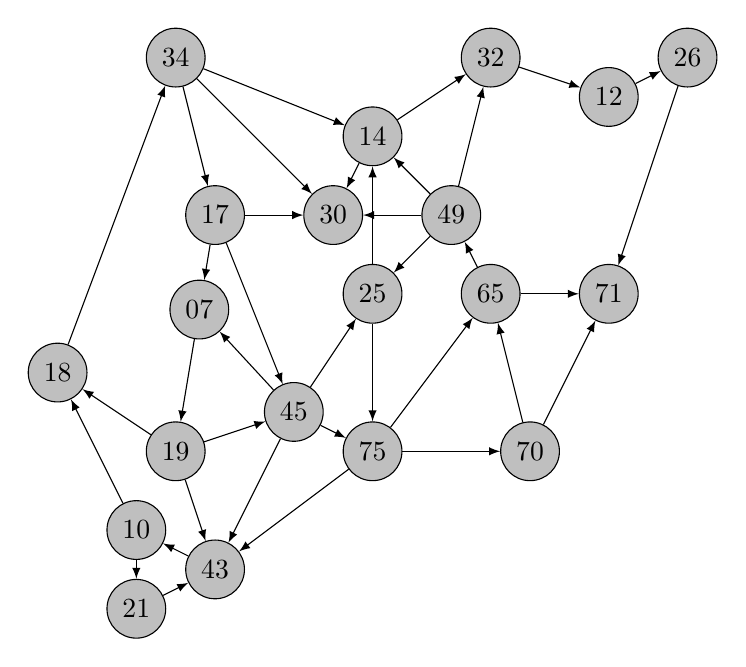
\begin{tikzpicture}
            \node[draw,circle,fill=gray!50] (21)at(0,0) {21};
            \node[draw,circle,fill=gray!50] (43)at(1,0.5) {43};
            \node[draw,circle,fill=gray!50] (10)at(0,1) {10};
            \node[draw,circle,fill=gray!50] (19)at(0.5,2) {19};
            \node[draw,circle,fill=gray!50] (45)at(2,2.5) {45};
            \node[draw,circle,fill=gray!50] (18)at(-1,3) {18};
            \node[draw,circle,fill=gray!50] (75)at(3,2) {75};
            \node[draw,circle,fill=gray!50] (70)at(5,2) {70};
            \node[draw,circle,fill=gray!50] (65)at(4.5,4) {65};
            \node[draw,circle,fill=gray!50] (71)at(6,4) {71};
            \node[draw,circle,fill=gray!50] (25)at(3,4) {25};
            \node[draw,circle,fill=gray!50] (07)at(0.8,3.8) {07};
            \node[draw,circle,fill=gray!50] (17)at(1,5) {17};
            \node[draw,circle,fill=gray!50] (30)at(2.5,5) {30};
            \node[draw,circle,fill=gray!50] (49)at(4,5) {49};
            \node[draw,circle,fill=gray!50] (14)at(3,6) {14};
            \node[draw,circle,fill=gray!50] (34)at(0.5,7) {34};
            \node[draw,circle,fill=gray!50] (32)at(4.5,7) {32};
            \node[draw,circle,fill=gray!50] (12)at(6,6.5) {12};
            \node[draw,circle,fill=gray!50] (26)at(7,7) {26};

            \draw[<-,>=latex] (75) -- (45);
            \draw[<-,>=latex] (75) -- (25);
            \draw[->,>=latex] (75) -- (65);
            \draw[->,>=latex] (75) -- (70);
            \draw[->,>=latex] (75) -- (43);
            \draw[->,>=latex] (45) -- (07);
            \draw[->,>=latex] (45) -- (43);
            \draw[->,>=latex] (45) -- (25);
            \draw[<-,>=latex] (45) -- (19);
            \draw[<-,>=latex] (45) -- (17);
            \draw[->,>=latex] (25) -- (14);
            %\draw[-,>=latex] (19) -- (10);
            \draw[->,>=latex] (19) -- (18);
            \draw[<-,>=latex] (19) -- (07);
            \draw[->,>=latex] (19) -- (43);
            \draw[->,>=latex] (43) -- (10);
            \draw[<-,>=latex] (43) -- (21);
            %\draw[-,>=latex] (43) -- (18);
            \draw[->,>=latex] (10) -- (21);
            \draw[->,>=latex] (10) -- (18);
            \draw[->,>=latex] (34) -- (17);
            \draw[->,>=latex] (70) -- (71);
            \draw[->,>=latex] (70) -- (65);
            \draw[<-,>=latex] (49) -- (65);
            \draw[->,>=latex] (49) -- (25);
            \draw[->,>=latex] (49) -- (14);
            \draw[->,>=latex] (49) -- (30);
            \draw[->,>=latex] (49) -- (32);
            \draw[<-,>=latex] (30) -- (14);
            \draw[<-,>=latex] (30) -- (34);
            \draw[<-,>=latex] (30) -- (17);
            \draw[<-,>=latex] (14) -- (34);
            \draw[->,>=latex] (14) -- (32);
            \draw[->,>=latex] (32) -- (12);
            \draw[->,>=latex] (12) -- (26);
            \draw[->,>=latex] (65) -- (71);
            \draw[<-,>=latex] (71) -- (26);
            \draw[->,>=latex] (18) -- (34);
            \draw[<-,>=latex] (07) -- (17);

        \end{tikzpicture}
    \end{center}

\end{frame}
\begin{frame}
    \frametitle{}

    \begin{framed}
        \centering Quelles variations du graphe orienté peut-on réaliser?
    \end{framed}

\end{frame}
\section{Graphe orienté}
\subsection{Définition}
\begin{frame}
    \frametitle{Graphe orienté - définition}

    \begin{aretenir}[]
        Dans un graphe orienté on ne peut parcourir les arêtes que dans un seul sens.
    \end{aretenir}
    \begin{center}
        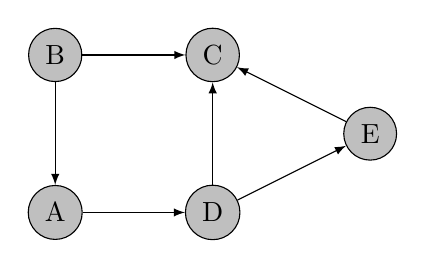
\begin{tikzpicture}
            \node[draw,circle,fill=gray!50] (A)at(0,0) {A};
            \node[draw,circle,fill=gray!50] (B)at(0,2) {B};
            \node[draw,circle,fill=gray!50] (C)at(2,2) {C};
            \node[draw,circle,fill=gray!50] (D)at(2,0) {D};
            \node[draw,circle,fill=gray!50] (E)at(4,1) {E};


            \draw[<-,>=latex] (A) -- (B);
            \draw[->,>=latex] (A) -- (D);
            \draw[->,>=latex] (B) -- (C);
            \draw[<-,>=latex] (C) -- (D);
            \draw[<-,>=latex] (C) -- (E);
            \draw[<-,>=latex] (E) -- (D);

        \end{tikzpicture}
    \end{center}
\end{frame}
\subsection{Degré d'un sommet}
\begin{frame}
    \frametitle{Degré d'un sommet}
    \begin{aretenir}[]
        On différencie les arêtes entrantes ($d^-$) et sortantes ($d^+$) d'un sommet.
    \end{aretenir}
    \begin{center}
        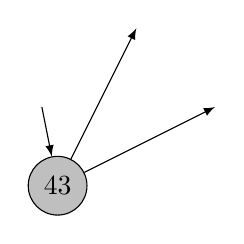
\begin{tikzpicture}
            \node[draw,circle,fill=gray!50] (43)at(1,0) {43};
            \draw[->,>=latex] (0.8,1) -- (43);
            \draw[<-,>=latex] (2,2) -- (43);
            \draw[<-,>=latex] (3,1) -- (43);

        \end{tikzpicture}
    \end{center}


\end{frame}
\begin{frame}
    \frametitle{}
    \begin{aretenir}[]
        La somme des degrés entrants et sortants d'un graphe est pair.
        $$\sum_{s\in S}{deg_+(s)+deg_-(s)}=2.A$$
    \end{aretenir}

\end{frame}
\begin{frame}
    \frametitle{}

    \begin{center}
        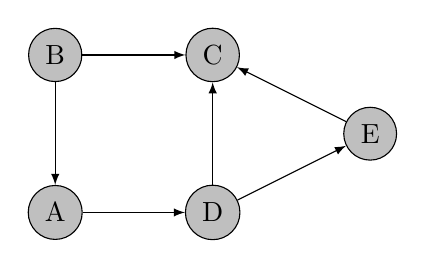
\begin{tikzpicture}
            \node[draw,circle,fill=gray!50] (A)at(0,0) {A};
            \node[draw,circle,fill=gray!50] (B)at(0,2) {B};
            \node[draw,circle,fill=gray!50] (C)at(2,2) {C};
            \node[draw,circle,fill=gray!50] (D)at(2,0) {D};
            \node[draw,circle,fill=gray!50] (E)at(4,1) {E};


            \draw[<-,>=latex] (A) -- (B);
            \draw[->,>=latex] (A) -- (D);
            \draw[->,>=latex] (B) -- (C);
            \draw[<-,>=latex] (C) -- (D);
            \draw[<-,>=latex] (C) -- (E);
            \draw[<-,>=latex] (E) -- (D);

        \end{tikzpicture}
    \end{center}
    \begin{activite}
        \begin{enumerate}
            \item Calculer les degrés entrants et sortants de chaque nœud.
            \item Calculer la somme des degrés.
        \end{enumerate}
    \end{activite}

\end{frame}
\begin{frame}
    \frametitle{Correction}

        \begin{itemize}
            \item A: $d^+=1, d^-=1$
            \item B: $d^+=1, d^-=1$
            \item C: $d^+=0, d^-=3$
            \item D: $d^+=2, d^-=1$
            \item E: $d^+=1, d^-=1$
        \end{itemize}
    \vspace{2em}
    $$\sum_{s\in S}{deg_+(s)+deg_-(s)}=12=2×6$$
\end{frame}
\subsection{Représentation en mémoire}
\begin{frame}
    \frametitle{Représentation en mémoire}

    \begin{aretenir}[]
        Dans une matrice d'adjacence, le sommet représenté sur la ligne est le départ de l'arête.
    \end{aretenir}
    \begin{multicols}{2}
        \begin{center}
            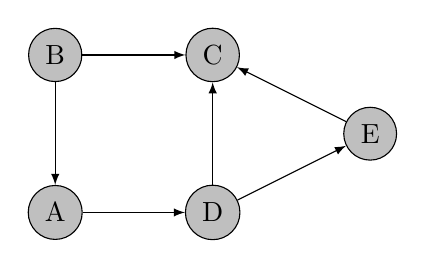
\begin{tikzpicture}
                \node[draw,circle,fill=gray!50] (A)at(0,0) {A};
                \node[draw,circle,fill=gray!50] (B)at(0,2) {B};
                \node[draw,circle,fill=gray!50] (C)at(2,2) {C};
                \node[draw,circle,fill=gray!50] (D)at(2,0) {D};
                \node[draw,circle,fill=gray!50] (E)at(4,1) {E};


                \draw[<-,>=latex] (A) -- (B);
                \draw[->,>=latex] (A) -- (D);
                \draw[->,>=latex] (B) -- (C);
                \draw[<-,>=latex] (C) -- (D);
                \draw[<-,>=latex] (C) -- (E);
                \draw[<-,>=latex] (E) -- (D);

            \end{tikzpicture}
        \end{center}

        $$\begin{pmatrix}
                0 & 0 & 0 & 1 & 0 \\
                1 & 0 & 1 & 0 & 0 \\
                0 & 0 & 0 & 0 & 0 \\
                0 & 0 & 1 & 0 & 1 \\
                0 & 0 & 1 & 0 & 0 \\
            \end{pmatrix}$$
    \end{multicols}

\end{frame}
\begin{frame}
    \frametitle{}

    \begin{center}
        \begin{tabular}{c|*{5}{c}}
              & A                      & B                       & C                    & D & E \\
            \hline
            A & 0                      & \cellcolor{LightGray} 0 & 0 &\cellcolor{SkyBlue} 1 & 0 \\
            B & \cellcolor{LightGray}1 & 0                       & 1                    & 0 & 0 \\
            C & 0   & 0                       & 0                    & 0 & 0 \\
            D & \cellcolor{SkyBlue}0                      & 0                       & 1                    & 0 & 1 \\
            E & 0                      & 0                       & 1                    & 0 & 0 \\
        \end{tabular}
    \end{center}
    \begin{aretenir}[Remarque]
        Dans un graphe orienté, la matrice d'adjacence n'est pas symétrique.
    \end{aretenir}

\end{frame}
\begin{frame}
    \frametitle{}
    \begin{center}
        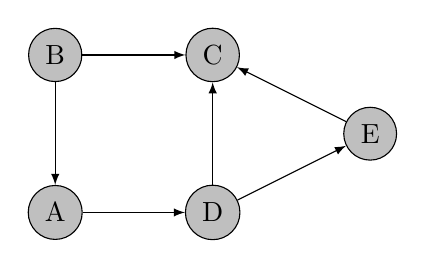
\begin{tikzpicture}
            \node[draw,circle,fill=gray!50] (A)at(0,0) {A};
            \node[draw,circle,fill=gray!50] (B)at(0,2) {B};
            \node[draw,circle,fill=gray!50] (C)at(2,2) {C};
            \node[draw,circle,fill=gray!50] (D)at(2,0) {D};
            \node[draw,circle,fill=gray!50] (E)at(4,1) {E};


            \draw[<-,>=latex] (A) -- (B);
            \draw[->,>=latex] (A) -- (D);
            \draw[->,>=latex] (B) -- (C);
            \draw[<-,>=latex] (C) -- (D);
            \draw[<-,>=latex] (C) -- (E);
            \draw[<-,>=latex] (E) -- (D);

        \end{tikzpicture}
    \end{center}
    \begin{activite}
    \begin{enumerate}
        \item Construire le dictionnaire des \textbf{successeurs} du graphe.
        \item Construire le dictionnaire des \textbf{prédécesseurs} du graphe.
    \end{enumerate}
    \end{activite}

\end{frame}
\begin{frame}[fragile]
    \frametitle{Correction}

    \begin{center}
    \begin{lstlisting}[language=Python , basicstyle=\ttfamily\small, xleftmargin=2em, xrightmargin=2em]
{"A": ["D"],
 "B": ["A", "C"],
 "C": [],
 "D": ["C", "E"],
 "E": ["C"]}
\end{lstlisting}
    \captionof{code}{Dictionnaire des successeurs}
    \label{CODE}
    \end{center}
    \begin{center}
        \begin{lstlisting}[language=Python , basicstyle=\ttfamily\small, xleftmargin=2em, xrightmargin=2em]
{"A": ["B"],
 "B": [],
 "C": ["B", "D", "E"],
 "D": ["A"],
 "E": ["D"]}
\end{lstlisting}
        \captionof{code}{Dictionnaire des prédécesseurs}
        \label{CODE}
        \end{center}
\end{frame}
\section{Graphe pondéré}
\subsection{Définition}
\begin{frame}
    \frametitle{Graphe pondéré - définition}

    \begin{aretenir}[]
    Dans un graphe pondéré, on donne un \textbf{poids} aux arêtes.
    \end{aretenir}
    \begin{center}
        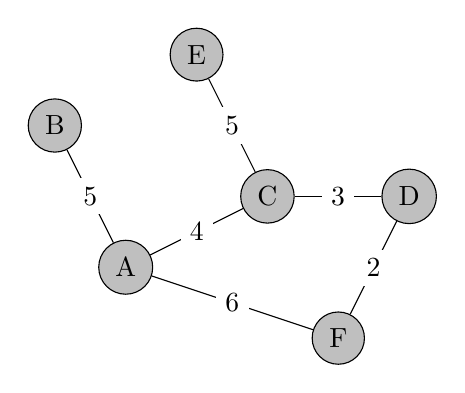
\begin{tikzpicture}[scale=0.9]
            \node[draw,circle,fill=gray!50] (A)at(0,0) {A};
            \node[draw,circle,fill=gray!50] (B)at(-1,2) {B};
            \node[draw,circle,fill=gray!50] (C)at(2,1) {C};
            \node[draw,circle,fill=gray!50] (D)at(4,1) {D};
            \node[draw,circle,fill=gray!50] (E)at(1,3) {E};
            \node[draw,circle,fill=gray!50] (F)at(3,-1) {F};
            \draw[-,>=latex] (A) -- (B) node[midway, fill=white] {5};
            \draw[-,>=latex] (A) -- (C) node[midway, fill=white] {4};
            \draw[-,>=latex] (A) -- (F) node[midway, fill=white] {6};
            \draw[-,>=latex] (C) -- (E) node[midway,fill=white] {5};
            \draw[-,>=latex] (C) -- (D) node[midway,fill=white] {3};
            \draw[-,>=latex] (D) -- (F) node[midway,fill=white] {2};
        \end{tikzpicture}
    \end{center}
\end{frame}
\subsection{Représentation en mémoire}
\begin{frame}
    \frametitle{Représentation en mémoire}
    \begin{aretenir}[]
    Dans la matrice d'adjacence, les valeurs non nulles représentent une arête avec un poids.
    \end{aretenir}
\begin{multicols}{2}
    \begin{center}
        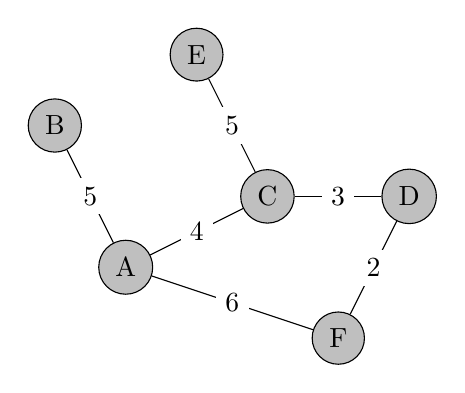
\begin{tikzpicture}[scale=0.9]
            \node[draw,circle,fill=gray!50] (A)at(0,0) {A};
            \node[draw,circle,fill=gray!50] (B)at(-1,2) {B};
            \node[draw,circle,fill=gray!50] (C)at(2,1) {C};
            \node[draw,circle,fill=gray!50] (D)at(4,1) {D};
            \node[draw,circle,fill=gray!50] (E)at(1,3) {E};
            \node[draw,circle,fill=gray!50] (F)at(3,-1) {F};
            \draw[-,>=latex] (A) -- (B) node[midway, fill=white] {5};
            \draw[-,>=latex] (A) -- (C) node[midway, fill=white] {4};
            \draw[-,>=latex] (A) -- (F) node[midway, fill=white] {6};
            \draw[-,>=latex] (C) -- (E) node[midway,fill=white] {5};
            \draw[-,>=latex] (C) -- (D) node[midway,fill=white] {3};
            \draw[-,>=latex] (D) -- (F) node[midway,fill=white] {2};
        \end{tikzpicture}
    \end{center}

    $$\begin{pmatrix}
        0 & 5 & 4 & 0 & 0 & 6 \\
        5 & 0 & 0 & 0 & 0 & 0 \\
        4 & 0 & 0 & 3 & 5 & 0 \\
        0 & 0 & 3 & 0 & 0 & 2 \\
        0 & 0 & 5 & 0 & 0 & 0 \\
        6 & 0 & 0 & 2 & 0 & 0 \\
    \end{pmatrix}$$
\end{multicols}
\end{frame}
\begin{frame}
    \frametitle{}

    \begin{center}
        \begin{tabular}{c|*{6}{c}}
              & A                      & B                       & C                    & D & E & F \\
            \hline
            A & 0                      & \cellcolor{LightGray} 5 & \cellcolor{SkyBlue}4 & 0 & 0 & 6 \\
            B & \cellcolor{LightGray}5 & 0                       & 0                    & 0 & 0 & 0 \\
            C & \cellcolor{SkyBlue}4   & 0                       & 0                    & 3 & 5 & 0 \\
            D & 0                      & 0                       & 3                    & 0 & 0 & 2 \\
            E & 0                      & 0                       & 5                    & 0 & 0 & 0 \\
            F & 6                      & 0                       & 0                    & 2 & 0 & 0 \\
        \end{tabular}
    \end{center}
    \begin{aretenir}[Remarque]
        Dans un graphe non orienté la matrice est symétrique.
    \end{aretenir}

\end{frame}
\begin{frame}
    \frametitle{}
    \begin{center}
        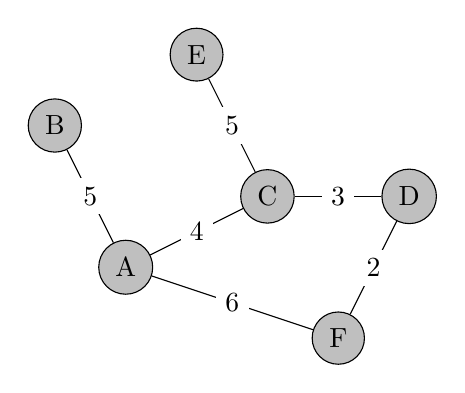
\begin{tikzpicture}[scale=0.9]
            \node[draw,circle,fill=gray!50] (A)at(0,0) {A};
            \node[draw,circle,fill=gray!50] (B)at(-1,2) {B};
            \node[draw,circle,fill=gray!50] (C)at(2,1) {C};
            \node[draw,circle,fill=gray!50] (D)at(4,1) {D};
            \node[draw,circle,fill=gray!50] (E)at(1,3) {E};
            \node[draw,circle,fill=gray!50] (F)at(3,-1) {F};
            \draw[-,>=latex] (A) -- (B) node[midway, fill=white] {5};
            \draw[-,>=latex] (A) -- (C) node[midway, fill=white] {4};
            \draw[-,>=latex] (A) -- (F) node[midway, fill=white] {6};
            \draw[-,>=latex] (C) -- (E) node[midway,fill=white] {5};
            \draw[-,>=latex] (C) -- (D) node[midway,fill=white] {3};
            \draw[-,>=latex] (D) -- (F) node[midway,fill=white] {2};
        \end{tikzpicture}
    \end{center}
    \begin{activite}
    Proposer une modification du dictionnaire d'adjacence pour prendre en compte les poids des arêtes.
    \end{activite}

\end{frame}
\begin{frame}[fragile]
    \frametitle{Correction}

    \begin{center}
        \begin{lstlisting}[language=Python , basicstyle=\ttfamily\small, xleftmargin=2em, xrightmargin=2em]
{"A": [("B", 5)],
 "B": [("A", 5)],
 "C": [("A", 4), ("D", 3), ("E", 5)],
 "D": [("C", 3), ("F", 2)],
 "E": [("C", 5)],
 "F": [("A", 6), ("D", 2)]
}
\end{lstlisting}
        \end{center}   
\begin{aretenir}[Remarque]
Cette solution n'est pas unique.
\end{aretenir}
\end{frame}
\end{document}